\documentclass[a4paper]{article}
\usepackage{graphicx}
\usepackage{mathtools}
\usepackage[a4paper, total={5in, 6.5in}]{geometry}
\usepackage{color}
\usepackage{tikz}
\usepackage{lipsum}
\usepackage{geometry}
\geometry{a4paper, left=2.5cm, top=2.5cm, bottom=2.5cm, right=2.5cm}
\usepackage{changepage}
\usepackage{booktabs}
\usepackage[font=small]{caption}
\DeclareCaptionFormat{mycaptionfont}{\fontsize{12}{13}\selectfont#1#2#3}
\usepackage{threeparttable}
\usepackage{ntheorem}
\usepackage{caption}
\usepackage{wrapfig,lipsum,booktabs}
\usepackage{listings}
\usepackage{pdflscape}
\captionsetup{format=mycaptionfont}
\usepackage{subcaption}
\theoremseparator{:}
\usepackage{lscape}

\usepackage[utf8]{inputenc}
\newtheorem{hyp}{Hypothesis}
\usetikzlibrary{shapes,decorations,arrows,calc,arrows.meta,fit,positioning}
\tikzset{
    -Latex,auto,node distance =1 cm and 1 cm,semithick,
    state/.style ={ellipse, draw, minimum width = 0.7 cm},
    point/.style = {circle, draw, inner sep=0.04cm,fill,node contents={}},
    bidirected/.style={Latex-Latex,dashed},
    el/.style = {inner sep=2pt, align=left, sloped}
}


\graphicspath{ {/home/angelo/Documents/Uni/Courses/Data Managment & Ethics/Integrated Assignment/assignemnet_project_folder/ERDs/} }


\begin{document}

\title{DME Integrative Assignment}
\author{Angelo Barisano; 508903 }
\date{September 30th, 2022}
\maketitle

\newpage




\section{Task 1: Plan \& Explore}

\subsection{Origin of Data \& Purpose Introduction}
Data drives security (Harrington, 2016). The wide spread adoption of data information systems has been used to recognize crime hot-spots to increase policing efficiency and protect people. However, the mere presence of a public repository of all crimes recorded in Chicago does not constitute effective use of data (Chicago PD, n.d.). As a consequence, this assignment is tasked with conducting an initial exploratory data analysis of the given data by utilizing a logical relational structure embedded in the raw data provided by the PD. This task will be achieved using SQL. Creating effective information systems and gaining insights for crime prevention is at the center of policy makers and executive branches of governments (Leenarts, 2018). 



\subsection{Purpose of this Assignment \& Data Plan}

To this end, a research database will be created in accordance to the FAIR principles (Findability, Accessibility, Interoperability, and Reuse) (Wilkinson, 2016). The expressed goal of this assignment is to offer a database and fundamental queries for data exploration; i.e. a database with flexible queries and insights meant for further analysis of the trends discovered in the data. Additionally, any code produced during this endeavour will be made public on GitHub for transparency reasons.\footnote{My private (non professional) github: $https://github.com/AngeloBarisano/data_management_and_ethics$} In the process of creating this assignment, the CESSDA data plan outline was used (Leenarts, 2018).

\paragraph{Data Description in Scope, Volume, and Format}
The data, provided by the Chicago PD, contains a sample of 730,900 registered crimes in the administrative districts of Chicago between the years of 2017 and 2021. The initial data source is in CVS-format and pertains to specific recorded crimes in the administrative jurisdiction of the Chicago PD in addition to time, location, crime type, and arrested or not. Thus, the data contact is to be found on the Chicago PD website (Chicago PD, n.d.). Considerations regarding the ethical (\& GDPR compliant regardless of whether the data comes from the USA) use of the data are aligned with the GDPR principles and, thus, FAIR (Wilkinson et. al., 2016).\footnote{Lawfulness, fairness and transparency, Purpose limitation, Data minimisation, Accuracy, Storage limitation, Integrity and confidentiality (security), Accountability} It is notable that, while this data is only a sub-sample of the total database crime data recorded in this time-frame, the overall trends in the data are still maintained. Thus, the EDA for which this database can be used for further analysing trends uncovered during this assignment. 

\paragraph{Project Time-frame, Researchers and overall Information} The set project time frame is the 27th of August 2022 till 2nd of October 2022. Involved in this project is only one student, Angelo Barisano.



\subsection{Research Question}
Upon conducting an initial Exploratory Data Analysis (EDA), three major data categories were identified in the raw data: 

\begin{itemize}
  \item Location
  \item Crime type
  \item Crime record data (time, arrest, etc.)
\end{itemize}

Based on the data categories and EDA, the following research questions guide the creation of the research database in increasing complexity. It may be noted, that the questions are meant to not be exact in their nature, but that the purpose of the assignment, database, and questions posed are of an explorative nature, evolving while answering said questions. Thus, this assignment is interpreted as an initial exploratory data analysis meant to uncover trends for further analysis in addition offering useful insights to policy makers. 

\paragraph{Question 1} Finding prevalent crime patterns in the data is a common starting point in exploring crime data. Crime trends take the form of temporal patterns distributed over a defined timeframe of interest. This kind of reporting is commonly used by policy makers (such as attorney generals) who are monitored based on their performance in terms of crime prevention and the overall trend that can be observed. 

Thus, this question provides future research with an adjustable query to gain an overview over the general distribution of crime by type. Subsequently applying a temporal component (i.e. by day of week, month, year, season, etc.) to this initial distribution reveals trends and temporal patters. This way, this question helps to answer questions to policy makers regarding general trends; such as how crime developed overall and by type (Harrington, 2016; Hickey, 2022). 

More importantly, however, the descriptive analysis of temporal patterns may uncover trends in the type of crime by time, which may be further examined in Q2 and Q3, using different dimensions. To this end, accessory dimensions will be integrated into the analysis to provide a holistic description. For instance assuming that crimes that lead to more arrests are more resource intensive, these crimes put a disproportionate strain on law enforcement. As such question 1 is supposed to be a broad exploration of the crime type by time:

\begin{itemize}
	\item What trends in by crime type can be observed in Chicago between 2017 and 2021? What are interesting categories of crime to be analysed further in Q2 and Q3?
\end{itemize}

This question will be answered by using a view which contains the date per crime in a convenient manner, such as year, month, day, hour. This way, the analysis is decreased in complexity; providing future researchers with easy to use time dimensions. Moreover, in this question, a variety of window function will be used to group by the time dimension and return a distribution per time component (e.g. year). 

\paragraph{Question 2} The next logical progression is to observe the location and crime dimension together. Certain crime trends, such as those uncovered in Q1, may be more localized; thus, certain neighborhoods and districts may be over-represented in certain categories. As such, in order to help the PD and policy makers to identify problematic areas with respect to certain crime hot-spots, districts and beats are analysed with respect to trends identified by the temporal component on a localized level. Thus, question two follows (again explorative):

\begin{itemize}
    \item Considering findings from Q1; how do the crime patterns wrt. crime type distribute by district? Is there a specific district which requires more attention?
\end{itemize}

This question will be answered similarly as Q1. However, the main focus here is laid on using standard $GROUP BY$ functions instead of window functions to demonstrate a variation in usage of SQL commands. 

\paragraph{Question 3} Finally, time, location, and crime type is triangulated. This enables policymakers to discern localized trends in the data in order to address crime patterns by distributing resources more efficiently; e.g. allocating more resources to dangerous beats during the night. Thus, by triangulating arrests by location and e.g. time of day this will enable us to show areas that need more attention by law enforcement.

\begin{itemize}
  \item Based on the sub-sample of trends uncovered in crime types in Q1 and their distribution by location in Q2; In order to deter crime, at what time of day might law enforcement allocate more resources to this location?
\end{itemize}

Overall, these project based questions are constructed in such a way that they guide an external user (PD) through the process of finding areas that need successively complex "sliced \& diced" information and culminate in the creation of actionable policy implications regarding prime prevention through resource allocation.

As such, by the descriptive and explorative nature of the questions posed, one can deduce that the entire analysis can be conducted using simple SQL functionalities.



\section{Task 2: Design and Organize}
The aforementioned questions in task 1 require three relevant data categories, as identified in the data. These pertain to the 1) time dimension, 2) location dimension, and 3) the crime or case instance itself. Generally, these already display common characteristics of regular entities in a relational database (Harrington, 2016). Thus, the design of the database followed the approach of combining logical structures (e.g. location) with an easy to use query design to explore the data.

We will start out with the case entity, as cases recorded in the original data create the centerpiece for all three posed questions.



\paragraph{Entity 1: Criminal Case} The first component consist of the individual instances of cases. Conceptually, these are central to this project as they enable the creation of the frequency distributions conditional on time and/or location. The variables that define this entity are as follows:

\begin{itemize}
  \item CaseId (natural key)
  \item DateTime object implicitly containing day, month, year, and time of day 
  \item Arrest Boolean  
\end{itemize}

These attributes are all atomic (DateTime objects are a technical solution and are, thus, atomic). Consequently, criminal case is by default in 2nd NF (also in 3rd NF). 

It may be noted that items such as location description and location themselves are not included in the final product in order to comply with the principle of data minimization (GDPR, 2018). This is also reduces the possibility of mistakes from occurring. 

The DateTime object will enable the clustering of crimes by the time dimension; which will be done via a view. Additionally, arrest information is used to further drill down the analysis and dissect the cases for more resource intensive cases. This is part of discerning interesting trends and exploring the data. The primary use case of case as an entity, however, is to make the entire database 1) work from a logical perspective (no crime distribution without each individual crime) and 2) to be the logical link between the type of crime committed in every case and where it happens. This way, the case entity is not only a natural entity, but it also fulfills the purpose of making the other two dimensions compliant to the 2nd and 3rd NF by default. Imagine that if we were to leave out case as an entity and immediately match crime types and location, the resulting two entities could not comply with 3rd normal form as crime types and location (as categories) would produce a many-to-many relationship - thus, not minimizing storage space, increasing query difficulty, and cause an inefficient relational database. As such, the case entity inadvertently functions as an associative entity, reducing many-to-many relationships to two many-to-one relationships.\footnote{I will not further elaborate on this; this is a logical conclusion; in order to reach 2nd normal form this is a required step which is obvious} As a consequence, case complies to the 3rd NF by definition as no stand alone entities are to be found in this entity (i.e. no transitive dependencies), while requiring the other data categories to normalize as well.\footnote{This definition of 3rd NF is far more intuitive and powerful (every entity in its own entity)}

In terms of the relation, IUCR and beat will be the foreign keys in this relation for them being natural (primary) keys in crime type and location respectively. Thus, criminal case is in 3rd NF.\footnote{This is actually an important insight of why many-to-many relationships pose problems wrt. normalization, data optimization and also query efficiency: in a query you would have to query on both tables simultaneously (which is possible but just annoying) while letting data explode because you need references (foreign keys) in both tables of the other table}

It is notable, that while such design choices should be reflected by leaving out case as an entity in the conceptual model in part 3 and then include it as part of the logical model, but case is too important to the functioning of the database in its purpose, that we will consider it along the way as a valid entity.
 
Please note that any datetime object should not get its own entity. This would violate rules set for relational databases as any instance created for case requires an instance to be creased in a datetime relation (Harrington, 2016); this would make the relation a one to one relationship, which are not efficient from a storage perspective. If the date dimension were to be split further into year etc, normalizing this structure would be not efficient from a query perspective; these problems are commonly solved by the ISO-Datetime format, which is why this dtype is atomic by definition.
 
Consequently, no problems of resolving many-to-many relationships are imposed on the design (i.a. no normalization issues later), while minimizing storage usage, in addition to adding an intuitive centerpiece to the database being implemented.  
 


\paragraph{Entity 2: Crime Type} Every criminal case requires a crime to be a valid instance. The raw data provides the IUCR, which identifies each unique combination of primary (e.g. homicide) and secondary crime category (e.g. first degree). Due to the latter two attributes being descriptions and categories, they are atomic. Thus, this relation is in 1st NF (and also 2nd and 3rd; see further down). The appropriate natural primary key is IUCR. 

Generally, most headlines only consider the primary type of crime, such as homicides, and generally disregard the secondary description of the data, such as first, second, or third degree in this case (Masterson, 2022). However, for certain crimes, such as homicide, it might be useful to be more differentiated wrt. e.g. gang related homicides. It is also the task of a FAIR database to enable future users to differentiate between different types of general crimes. Furthermore, it might be the case, that certain subcategories of crimes tend to be more prevalent than others.
Subsequently, due to the inclusion of the secondary description of the crime, this necessitates that crime type is an entity on its own in order for criminal case to comply with 3rd NF. \footnote{if only primary type would have been included, it would have been correct to include it in the criminal case entity} Suppose only the primary category of any crime committed was to be analysed. This would imply that both the IUCR and secondary description would be superfluous. Subsequently, any entity with only one variable is a superfluous entity, taking up unnecessary storage space (similar to one to one relationships). The reason for this is that if a crime occurs, a foreign key would have to relate the primary crime type to the crime type entity. Obviously, the primary crime type foreign key would be the only variable (and primary key) in crime type. As such, it would not make sense from a relational perspective to split crime type into a separate entity. It would make more sense to integrate it directly into the case entity. However, now, due to the inclusion of secondary description as an attribute, crime type has to be its own entity in order to move the case table from 2nd to 3rd normal form (the crime type information would not be transitive). Subsequently, the creation of a crime type entity moves both the case entity and crime type entity into 3rd normal form. Moreover, IUCR then becomes a natural PK (and FK) in this relationship. Subsequently, through the initial design choice, any issues regarding normalization are being taken care of. 


\paragraph{Entity 3: Location} Finally, the location information is being considered. Here, a similar logic applies as with the crime type. In order to analyse certain administrative boundaries, such as districts etc., a location entity has to be included. Hypothetically, if we were to only include information in the database pertaining to in which district an instance of a crime was recorded, the aforementioned case entity would be the most optimal place for such a variable to be stored. However, this research database aims at offering the ability to further analyse certain subsections of particular police districts - their beats in order to offer better descriptive results. 
Subsequently, any instance of a crime recorded will have its district and beat included. Following hierarchically, beats are below district; one district containing multiple beats. This implies that the most optimal database structure is to use beat as the primary and foreign key in this relationship. This way, any normal form issues are resolved by default, setting both the case and location entity into 3rd normal form. 

The reason to exclude block as a entity of analysis is twofold. 1) blocks overlap to some extend with different districts and beats increasing the level of analysis unnecessarily. 2) Beats and districts are administrative units, while blocks require local knowledge, which is what we try to use to answer for the aforementioned questions. 


\paragraph{Logging \& Master Table} Finally, a small master table will be included which tracks any information regarding formatting the data, data retrieval, and restrictions/ triggers called (not included in part 3 due to relevancy). Such relations are not part of the standard relationship model and are, thus, excluded from the ERD development in part 3. 


\paragraph{Conclusion} Based on the questions posed during task 1 in addition to the fundamental nature of the data provided, the structure described in this section offers an intuitive optimal solution for any normal form problems that might arise. Particularly the inclusion of the case entity as an integral part of the relationship model automatically resolves any issues pertaining to the inclusion of location and crime type information on a case by case level; all entities are by definition in 3rd NF given the available data.\footnote{I assume that this is clear: if there would for instance be more info about each beat and district individually, then location would not be in 3rd NF. So this statement is based on the availability of the included data.} 

\pagebreak


\section{Task 3: ERD}



\begin{figure}[htp]
		\centering
		\includegraphics[scale=.40 ]{ConceptualDiagram.drawio.png}
         \small
         \caption{Conceptual Diagram}
\end{figure}



\subsection{Conceptual Model}
As mentioned in part 2, the individual criminal case instance is central to the database design. Contemporaneously, the case entity resolves all problems regarding normal form (all tables are in 3rd NF) and many-to-many relationships. Subsequently, the conceptual model describes the relation of the three entities described in part 2: 

\begin{itemize}
  \item Location
  \item Case
  \item Crime Type
\end{itemize}

\indent Disregarding information regarding keys, the structure outline in part 1 \& 2 is described here from left to right. To start with, the location entity describes where any crime instance is taking place in terms of beat and implicitly the corresponding district. Consequently, location is related to criminal case with a one (non-mandatory) to many (mandatory) relationship, red from left to right. 
The reason for this specific choice of cardinality is simple: in order to be included in the data, a district or beat must have had at least one crime happening in it; otherwise it would not show up in the raw data. As we are not creating a true transnational database, but rather a research project database, we do not have to care for the hypothetical case of a district being included just to make sure you can create future crime instances in this specific location instance. In order to be included in the raw data, a location (be it beat or district) must have experienced at least one crime instance. Thus, for this specific case of a research project driven database, the $model$ is requiring any location to have at least one crime instance. A similar argument will be used further down as well for crime type. Contrarily, certain crimes do not have a location; think of financial crimes. It would be wrong to remove these records. Thus, a criminal case instance does not need a location.

\begin{itemize}
\item As such this is then read as: one location must have experienced at least one or many criminal cases; One criminal case can occur in one and only one, but not mandatory, location instance.
\end{itemize}

\indent Subsequently, we need the criminal case entity, which contains all case related information on an individual subject basis. Continuing to the right of it, case and crime type is related via a mandatory one to many and mandatory one and only one relationship. Crime type gives the general description to each criminal case (description is the same as in part 1 and 2). The choice for this cardinality is similar to the aforementioned relationship. A criminal case must have a crime type, otherwise it is invalid as no crime would have been committed. Contrarily, a crime type, in order to be included in the initial raw data, must have been committed once at least. This is actually the case here. Certain IUCRs, which exist in the penal code in Illinois, were not committed and are thus not included in the raw data file.
\begin{itemize}
\item As such this is then read as: one criminal case pertains to one (mandatory) and only one crime type; one crime type can be perpetrated in one or many (mandatory) criminal cases.
\end{itemize}

\paragraph{Intermezzo:} It may be notable that the model shows mandatory relationships for crime type and location. Technically correct would be to use non mandatory relationships for location and crime type. For example a district or crime may not have been perpetrated and, thus, would not have a record. This research does not consider this case as the goal of this data base is to use the existing data for analysis. As such, in order for a district/ crime to be included in the database, a crime instance must have been created for these instances. As such, the choice was made to include a mandatory relationship for these cardinalities.

\subsection{Logical Model}


\begin{figure}[htp]
		\centering
		\includegraphics[scale=.40 ]{LogicalDiagram.drawio.png}
         \small
         \caption{Logical Diagram}
\end{figure}

Figure 2 describes the logical model. For location, "beat" is chosen as primary key because beat (as a stand alone entity) would be hierarchically below District; one district - many beats. As such, each district is uniquely identifiable by its beat in case we want to aggregate, which is why beat is the only natural (primary) key in this relation. In reality (with more variables in location) this relation is not in 3rd normal form as district is usually an entity on its own. However, due to no more data/ variables being available on beat or district, this relation does not contain any transitive dependencies and is, thus, in 3rd NF. The meaning of each attribute here is self explanatory. More importantly, the primary key beat is in TEXT form (also district). The reason for this is that beats are defined in the first two characters by their district and the latter two describe the beat. Thus, a beat instance may start with a "0". In many scripting languages and some databases, this leads to problems and the removal of the "0", as the underlying software does not interpret the "0". As such, TEXT was chosen for data quality reasons. Please note that the same argument applies to crime type and IUCR. 

\indent Following, CrimeID was chosen to be the primary key of case, due to it being a natural primary key. This is a standard auto-incremental integer key and can, thus, be treated as an integer; though care should be applied when reading the data into scripting languages. In addition to each CrimeID identifying each instance of a crime committed, DateTime and Arrest are included as attributes. DateTime has TEXT as dtype as SQLite does not support a conventional datetime object, which then defaults to a string value. DateTime provides year, month, day, hour, minute, second of the instance 8as any other datetime dtype does by definition). Arrest has the dtype TEXT for a similar reason (safety); SQLite does not support Boolean dtypes. A possible alternative would have been to use 1 or 0, but a simple string input TRUE or FALSE has the same functionality in the and while being more explicit. Arrest describes the state of each criminal case whether or not an arrest was made. 


\indent Finally, crime type's primary key is the IUCR key, a natural primary key. It uniquely identifies each crime category plus its secondary description. Its dtype is TEXT for the same reason as for why beat's dtype is TEXT. Following, primary category has dtype TEXT and ´describes the overall category of the crime committed. Secondary category then further describes each primary category; thus, it also has a TEXT dtype. 



\subsection{Physical Model}


\begin{figure}[htp]
		\centering
			\includegraphics[scale=.40 ]{PhyscialDiagram.drawio.png}
         \small
         \caption{Physical Diagram}
\end{figure}

As mentioned in part 2, the inclusion of case as a full entity throughout the entire process automatically removes any many-to-many relationships. Additionally, this simplified the choice in appropriate foreign keys to describe the relationships. Remember, foreign keys must be placed in the adjacent entity on the many side (the other way around would be counterproductive). Thus, beat is the foreign key in criminal case for location and IUCR is the foreign key in criminal case for crime type. The reason for this should be self explanatory. It may be noted that CrimeID is still the unique identifier in criminal case as it is unique by its own right. 

Thus, planing in part 1 and 2 simplified this part considerably by default. 


\section{Task 4: Data Quality checks and preparation}

In the process of preparing the data to be loaded into the research DB, python was the scripting language of choice. For transparency reasons (FAIR) the data preparation file is contained as an attached file. 

In order to conduct the data cleaning, the GDPR's dataminimization and quality principles were applied (the others, though important, are less applicable here) (GDPR, 2018). Dataminimization states that only data that is actively being used and has a purpose of being stored should be included in a database. While this project is based on a public database from the US (so technically GDPR does not apply; particularly because no individual is identifiable), GDPR still offers guiding principles/standards on how to fair with data. Additionally, dataminimization has a practical usage point: less data means fewer errors.\footnote{Please note that I studied the GDPR at UvA and had to work with it; so I can speak from experience.} Thus, not all data in the raw data is included. This also means that considerations regarding FAIR were made (see part 1).  


\

Generally, the data quality of the provided  raw sample is very good; less than 0.01\% of observations display any anomalies. This is attributable to the origin of the data being of administrative nature by public offices.

\indent The operations performed specifically relate to the relevant data for this endeavour mentioned in part 3. Firstly, 3 instances contained no case numbers. These records were broken overall and were, thus, removed. Secondly, 16 instances missed date. As date is a central to the analysis, these records have to be removed. Moreover, 79 instances had non-correspondent beats and districts. While it would have been possible to impute the missing data based on the block or lat-lon information, one must assume that all location related information wrt. these observations is compromised. Similarly as before, location quality is central to answering the questions in this assignment; thus, these instances were removed. Finally, 149 perfectly duplicated items were removed. 

\indent In terms of data transformations, date was transformed into SQL castable form to run functions on date (correcting for AM and PM and correcting the string inputs). Moreover, beat and district instances were repaired wrt. the preceding "0" filler, creating instances of length four and two respectively. Finally, arrest ("true", "false") was cast into Boolean form. 

\indent Regarding non-crucial anomalies, 15 instances miss arrest; but this information is only used for one sub query once, which is why it was kept. Additionally, seven records of case numbers display noncompliance. However, CaseID is a perfect reflection for this issue. Considering CaseID, set-tests (looking for duplicates in a set object) were conducted to warrant that no IDs were missing beyond the removed records. Further, one instance of lat-lon showed an extreme outlier which was converted to NaN, due to the beat and district information appearing properly. It may also be notable that the absence of information is still information; i.e. financial crime might not have a location (refer to part 3 discussion of cardinalities). 

Overall, the consequences of removing these observations is minimal. Of a total of 730900 observations, we were left with 730654 records. 

Finally, considering crime type related data, secondary description and through that IUCR, contained typos, resulting in duplicated values. However, the typos did not change the meaning of the secondary descriptions. As such, a simple merge-right-join was performed to drop all duplicates on that dimension without loosing any data.

\section{Task 5: Create Tables and Load the Data}

Please note: Execute the tabs in SQL in the exact order I upload them. This is needed for the views and triggers to function properly.

\
Upon implementing the physical ERD into SQL, location and crime type (implemented as crime type for convenience when querying) the $CREATE TABLE$ command was used. Beat and IUCR were defined as PK using the $PRIMARY KEY$ command. The $UNIQUE$ + $NOT NULL$ constraint are technically not needed due to the designation of these attributes as PK. They were, however, included to be explicit and clear. Moreover, $NOT NULL$ was applied to the district attribute and primary category (implemented as PrimaryCategory for convenience in querying) as these should not be empty following their definition in part 3. However, secondary category (implemented as SecondaryCategory) in crime type did not need these restrictions as certain primary types may not have a secondary category.

Following, the criminal case relation (implemented as CriminalCase) contained the only $FOREIGN$ $KEY$ restrictions as described in part 3. Considering constrains implemented wrt. the relations (through foreign keys), upon update and deletion, all related instances in the parent table should be removed: i.e. $CASCADE$ update and deletion (one only implements these on the foreign keys to signal SQL how to conduct such operations). The reason for this is twofold: 1) in a usual transnational database, such operations should be restricted as no human should have writing access to a specific instance (Harrington, 2016). However, we are dealing with a research project database; as such, it might be the case that it turns out that one district instance should not exist (is erroneous). As such, all "supposed" crimes that happened in this district would have to be removed. That is why cascade deletion was chosen. Following, CaseID was the optimal primary key choice; a $NOT NULL$ restriction was only implemented on the date attribute (and of course CaseID) as outlined during part 3 (date is required)

Finally, a small $CHECK$ was implemented in order to control whether loaded instances comply with the time dimension.\footnote{No "if exists" table creation was implemented as this is bad practice.}

Finally, in order to load the data, $INSERT INTO$ commands with $DISTINCT$ operations were used. 

Regarding the master table and logs, a master table was creates containing the ID attribute to record the IDs of the instances mutated, in addition to a datetime class and a transaction report (what has been done). This table is not related to the model as a whole.



%https://www.sqlshack.com/learn-sql-sql-triggers/
%https://www.sqlitetutorial.net/sqlite-foreign-key/
%https://www.crewmachine.com/use-mysql-triggers-recording-history/



\section{Task 6: Analysis}
Please note that I cannot describe all queries completely. Scalar functions, analytical functions, window functions, and joins are used in abundance throughout the analysis. Moreover, the attached python file shows the process of visualization using SQL to feed into a scripting language. Furthermore, the database was $VACCUMED$ before submission. 
Additionally, the database was not saved directly in the repository due to security concerns (.gitignore). Also, no virtual environment was set up to facilitate the project. Finally, it is notable that in order to answer the questions, multiple different approaches in writing the queries were chosen, ranging from joining sub queries to window functions in order to demonstrate knowledge of all functions. Additionally, I wanted to try the speed of different styles of code (particularly the procedural generated optimization behind window functions).

\subsection{Question 1:}

Note: Please execute every query one by one in this tab.

The first question considered how overall crime patterns are distributed with respect to the temporal component. To this end, a view containing transformed datetime by crime case  outputs was constructed as it would be of use throughout this project ($CREATE VIEW$. This query utilized a sub query which used the $STRFTIME$ string parser to obtain year, month, day, hour from every crime case instance. Subsequently, the $CAST$ function was used to cast hour/ time of day into morning, noon, evening, night buckets per instance, creating a convenient view to analyse different dimensions of time per each crime (see ViewTab).


\paragraph{Part 1} Consequently, the first sub-question considered what the overall trend in crime was per year; i.e. are total crime levels increasing or decreasing? This question is relevant for public officials, which are held responsible for overall crime levels. 

In order to answer most questions in question 1, a multitude of analytical window functions was used. For this question two queries were produced: 1) Based on the aforementioned view on time, a $GROUP BY$ was performed on year to $COUNT$ all crime instances per year. This query was used as a sub query in a query using a $LAG$ window function in combination with some casting to calculate the change to the previous year. 2) Utilized the same query, but extended it with a $WHERE$ clause to calculate the total change in crimes over the years (see Question 1 tab part 1).

As can be seen in \textbf{Figure 4 a)} overall crime levels reduced during the observation time-frame of 2017 to 2021. In 2017, the overall level of crimes recorded was at 161304, which gradually reduced to 124558 crimes committed. Overall, this resulted in a reduction of 22.78\% in total crimes recorded. Thus, on a superficial level, crime tends into the right direction. 


\paragraph{Part 2} However, overall crime levels do not consider the severity of the crime committed. In this context, this analysis focuses on resource intensive crimes as a subset. This subset was defined by calculating the proportion of attests in this specific overall (primary) category. It was decided due to brevity concerns that if a crime category displayed more than 50\% arrest rate in addition to more than 500 total arrests over the period of the five recorded years (100 per year), that this crime poses a reasonably higher strain on law enforcement; this is because if such a crime occurs, two law enforcement officers have to respond only to arrest the suspect in question and bring it to jail while not being able to respond to other calls and if they occur not frequently enough they do not pose a strain on law enforcement. 

In order to achieve this, another view was created (resource intense; see view tab). This view used multiple $JOIN$ statements joining two queries and multiple tables in those sub queries with a $ROUND$ function to calculate the proportion of arrest to total crimes committed per primary category of crime (see view tab). Secondly, this view was used in the primary query for this part, which joined in a sub query on this view in order to sub-sect the data by the the specification above and then again applied a $LAG$ window function over two partitions (primary category and year) to obtain the total crimes committed and percentage change to previous year per primary crime category ordered by year. Overall, of the 34 primary categories defined in the data seven fulfill this classification.Figure 4 b) shows the development over time of these categories. Primarily, while increasing initially, Narcotics related crimes dropped by 56.92\%, posing the most frequent category in this category, starting at 6946 in 2017 and dropping to 2992 records. The largest reduction was observed in Prostitution related crimes from 438 in 2017 to 53 in 2021, which constitutes a reduction 89.90\%. Finally, the only category that showed an increase in this subcategory was Weapons Violation, which displayed an increase of 93.89\% from 2814 to 5456 recorded crimes. Overall, resource intensive crimes showed an overall drop of 29.95\% from 15958 to 11178. Combined with the insight that overall crime levels have dropped, this implies that law enforcement is less strained in 2021 than in 2017. 



\paragraph{Part 3} When considering all crime categories again, the question which categories, regardless of whether they are resource intensive or not, have shown the largest rise and reduction my be considered. This was achieved by utilizing all aforementioned queries and time view in two large queries which used a window function to $DENSE_RANK()$ and $OVER(PARTITION BY PrimaryCategory)$ crimes by the total change over the entire timeframe $LIMIT$(ing) the output once to the five crimes with the largest decrease and once to the five crimes with the largest increase by  (see tab Question 1 part 3). Figure 5 a) displays the top five categories with the largest reduction, while Figure 5 b) shows those categories with the largest increase in records. While the overall trend was positive in terms of over crime levels reducing, crime categories such as Homicide and Human Trafficking show a 19.94\% and 80.0\% increase respectively. When analyzing homicides related crimes, it may be interesting to subsection by secondary type in order to obtain an understanding what constitutes this crime type. Considering for instance homicide, one can see that of the two existing categories (reckless homicide, first degree homicide), first degree homicides clearly dominated (by a ratio of at least 100 to 1) and that first degree homicides increased by 20.68\%. This implies, that while the overall trend in the crime is positive, certain subcategories display a severe increase.  



\begin{figure}%
    \centering
    \subfloat[\centering Total Crimes Recorded]{{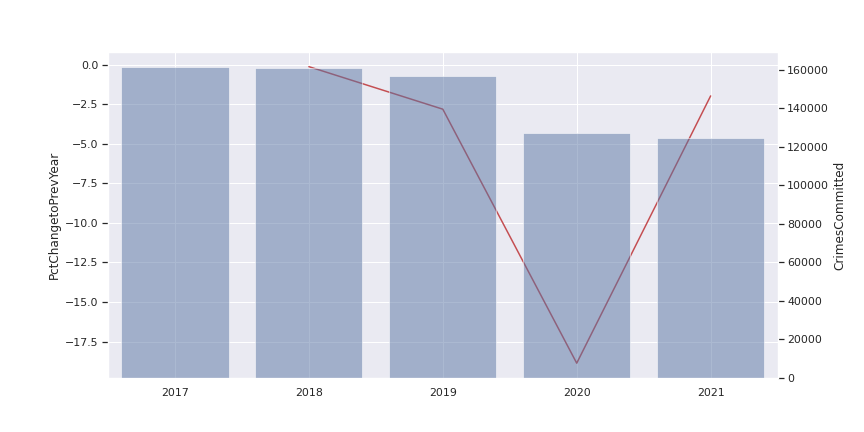
\includegraphics[width=7.5cm]{/home/angelo/Documents/Uni/Courses/Data Managment & Ethics/Integrated Assignment/assignemnet_project_folder/Code/q1_part1.png} }}%
    \qquad
    \subfloat[\centering Resource intensive Crimes Annual Change]{{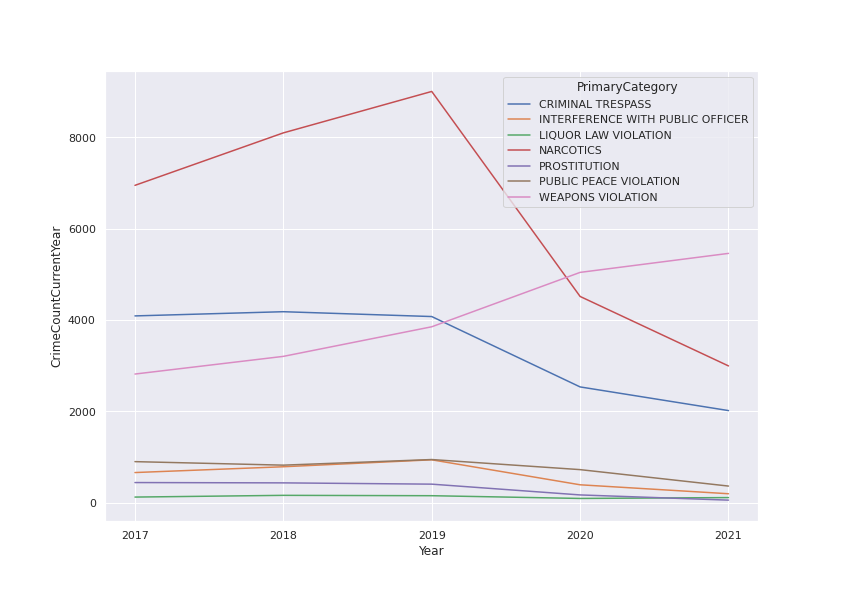
\includegraphics[width=7.5cm]{/home/angelo/Documents/Uni/Courses/Data Managment & Ethics/Integrated Assignment/assignemnet_project_folder/Code/q1_part2.png} }}%
    \caption{Temporal Component \& intensity and Crime by Category}%
    \label{fig:example}%
\end{figure}


\begin{figure}%
    \centering
    \subfloat[\centering Crime Categories with the greates Reduction]{{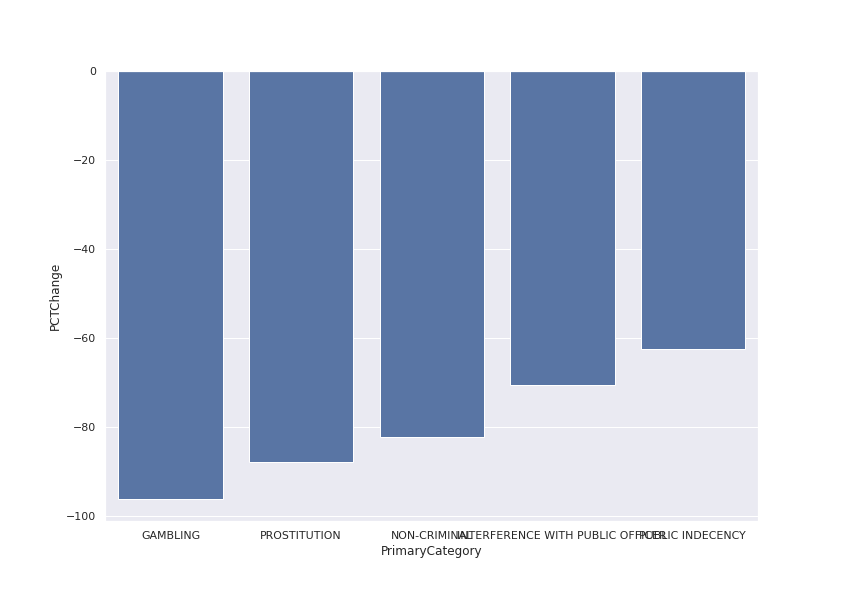
\includegraphics[width=7.5cm]{/home/angelo/Documents/Uni/Courses/Data Managment & Ethics/Integrated Assignment/assignemnet_project_folder/Code/q1_part3a.png} }}%
    \qquad
    \subfloat[\centering Crime Categories with the greates Increase]{{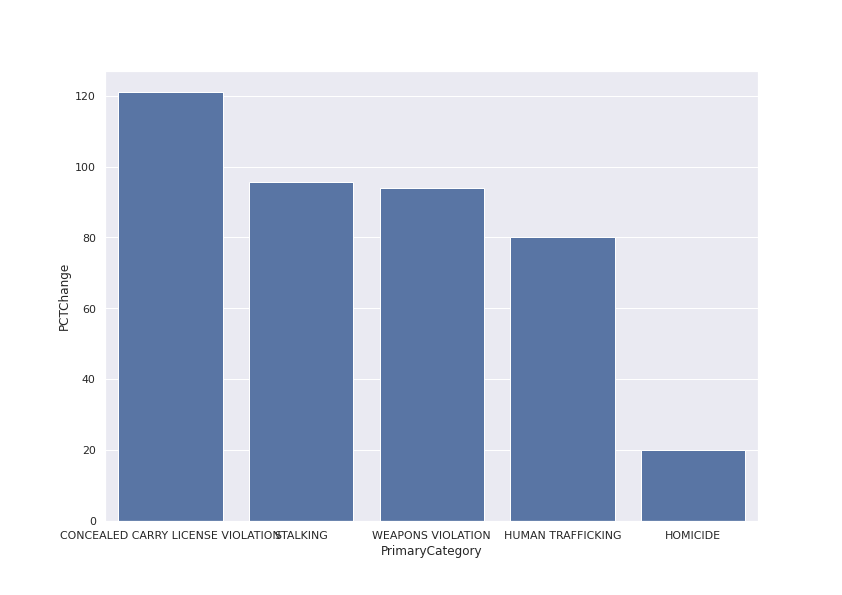
\includegraphics[width=7.5cm]{/home/angelo/Documents/Uni/Courses/Data Managment & Ethics/Integrated Assignment/assignemnet_project_folder/Code/q1_part3b.png} }}%
    \caption{Total Change in Crimes committed by category 2017 - 2021}%
    \label{fig:example}%
\end{figure}




\subsection{Question 2:}


When considering the following primary crime types 'homicide', 'prostitution', 'weapons violation', 'narcotics' from question 1, these crimes show interestingly large changes to be used as further subsections. Subsequently, question 2 considers which locations are predominant in these crime types. 

After identifying interesting primary types of crimes by time aspect, it is now relevant to sub-sect the data further by district in order to identify problem districts. To this end, a (large) query was used which uses multiple scalar functions, nested queries and window functions, and a left join plus multiple inner joins and cast functions (this query is too difficult to describe)

The goal was to create a ranking based on the total proportion of the primary category crimes identified ('homicide', 'prostitution', 'weapons violation', 'narcotics') in question 1 per district, limiting the results to the top three districts per crime category. To this end, a (large) query was used which uses multiple scalar functions, nested queries and window functions, and a left join plus multiple inner joins and cast functions (this query is too difficult to describe). It started out in a sub query which calculates the total crimes committed per primary category using two join statements. Next, a sub query was created which also used conventional group statements to calculate the primary crimes committed per district. The first query was then left joined onto the second query, as the first sub query contained only the overall totals per category, which then had to be cast to the dimensions of the second query using a $LEFT JOIN$ (see question 3 answer for a shorter approach). Finally, a $DENSE RANK()$ and $OVER(PARTITION BY PrimaryCategory)$ was used to rank each primary category by its proportion in total crimes committed and limit the output to three districts per primary crime category (see Question 2 tab).

Table 1 reports the result of this query.\footnote{see attached python file for stargazer output generation} What is striking (I was surprised myself): in all crime categories that saw the largest movement over the years, district 11 is in at least the top three for each crime category. Consequently, district 11 must be monitored more closely. When performing a similar subset analysis as in Q1 wrt. homicide but now by beat, one can see that there is little difference in homicide and other categories by beat, which is why district 11 will be used as the level of analysis in Q3. 

\begin{table}[!htbp] \centering 
\begin{adjustwidth}{0cm}{-0cm}
\begin{threeparttable}
\small
\captionsetup{font=small, justification=raggedright,singlelinecheck=false}
\caption{\textsc{Districts Ranked by Proportion of Crimes Committed}}
\centering 
  \label{}
\small 
\begin{tabular}{@{\extracolsep{8pt}}llrrr} 
\\[-5.8ex]\hline 

\toprule
  Prim.Cat. & District &  Rank &  Tot.Crimes District &  PCT Crimes committed Category\\
\midrule
         HOMICIDE &       11 &                     1 &                          211 &                   11.32\% \\
         HOMICIDE &       06 &                     2 &                          178 &                    9.55\% \\
         HOMICIDE &       05 &                     3 &                          153 &                    8.21\% \\
        NARCOTICS &       11 &                     1 &                        10157 &                   32.20\% \\
        NARCOTICS &       10 &                     2 &                         3540 &                   11.22\% \\
        NARCOTICS &       15 &                     3 &                         2194 &                    6.95\% \\
     PROSTITUTION &       11 &                     1 &                          856 &                   57.37\% \\
     PROSTITUTION &       07 &                     2 &                          179 &                   12.00\% \\
     PROSTITUTION &       05 &                     3 &                          132 &                    8.85\% \\
WEAPONS VIOLATION &       07 &                     1 &                         2190 &                   10.76\% \\
WEAPONS VIOLATION &       11 &                     2 &                         2185 &                   10.73\% \\
WEAPONS VIOLATION &       06 &                     3 &                         2023 &                    9.94\% \\
\bottomrule
\hline \\[-3.5ex] 
\end{tabular} 
\begin{tablenotes}[para,flushleft]
      \small
      \item\textit{ }
    \end{tablenotes}
\end{threeparttable}
\end{adjustwidth}
%
\end{table}

 



\subsection{Question 3:}



Finally, considering district 11 from Q2 in combination with the relevant crime categories from Q1, we will examine both dimensions together to answer how to potentially counter these trends productively from a resource perspective. To this end, each category is split into when it occurs during the day (morning, noon, evening, night).
To gain this insight, a concise query was created that merges all approaches from question 1 and question 2 into one concise version. Based on the time of day view, four JOIN statements were performed, bringing the entire database together and then a window function using $SUM$ and partitioning over primary crime category was used to calculate the proportion of crime by time of day per primary type category (see Question 3 tab).
Figure 6 displays a stacked bar-plot to visualize the distribution of crimes within each category by time of day for district 11. This plot can now be used to analyse how to actively counter a specific crime category. One such example would be to deploy more units during evening (18-24h) to deter prostitution related crimes. It may of course be noted that a higher presence of law enforcement would lead to more arrests and more records being created of crimes. Non-recorded crimes are obviously not included in the data (simultaneous causality). As such, no claim regarding causality is being made during this assignment as only general trends are reported in form of an exploratory data analysis. Additionally, the data was randomized. However, the process in generating this insight has been noted and can be reused. The adjacent python file contains the queries and casts into dataframe in order for future research to continue this endeavour. 


\begin{figure}[htp]
		\centering
			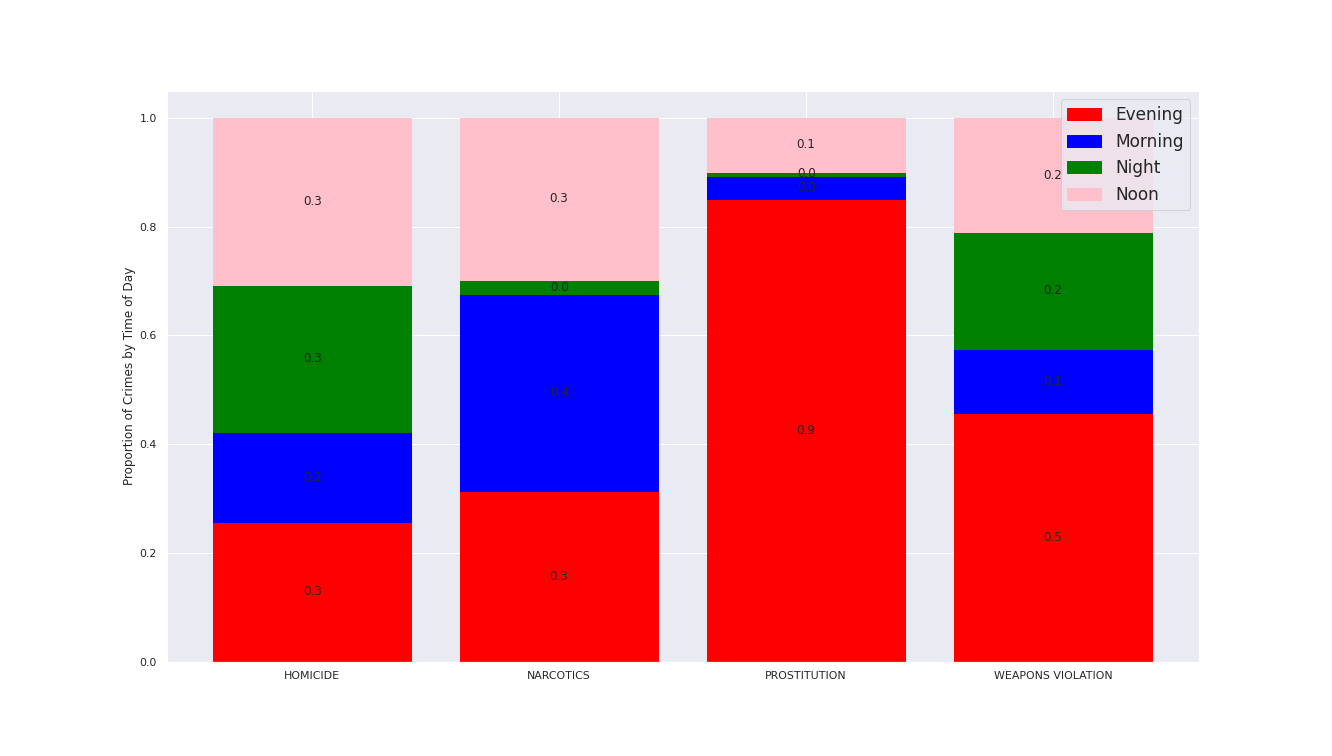
\includegraphics[scale=.35 ]{"/home/angelo/Documents/Uni/Courses/Data Managment & Ethics/Integrated Assignment/assignemnet_project_folder/Code/q3.png"}
         \small
         \caption{Proportion of Crime committed by Time of Day for District 11}
\end{figure}



\subsection{Use of Triggers and Indexes}
\paragraph{Triggers:} Two triggers were created. 1) an insertion log trigger on the criminal case entity ($CREATE$ $TRIGGER$), which logs the IDs of new crime cases. This trigger has a practical purpose of ensuring data integrity (GDPR, 2018). I have personally used such triangulation tables to ensure that no instance was wrongfully included or is missing. The way such a log is used is that whenever transformations are done outside of the database, one can always verify the integrity by checking on a set of IDs (here CrimeIDs) which is the fastest way of controlling for missing data after a transformation. This way, during certain analyses, missing records can be funneled through special automated tests (Harrington, 2016). However, this goes beyond the scope of this assignment. Consequently, this trigger was already applied, as it recorded every CrimeID loaded into the criminal case entity at the very beginning.
2) based on the CASCADE deletion restriction on Criminal Case, it might happen that upon a deletion of a certain district (hypothetically), any criminal case related to this district is dropped as well. Assume, a district was added by mistake. You want to delete this district (which should be possible in a research DB). However, you make a mistake and delete another district, which then removes a cascade of other data in Criminal Case. By logging all deletions in the master table, these drops can be easily recovered from a backup and inserted back into the database.
\paragraph{Index:} In total, three indexes were created. Of these, two are of particular importance as they are continuously used in Q2 and Q3. 1) index on district 11, indexing on location and on district 11 for demonstration purposes mostly. It was created using the $CREATE INDEX$ command, followed by the specification of the location table and a WHERE clause on district == 11. 2) the second index on the primary category sub-types discussed in Q2 speeds up the query speed in Q2 and Q3. It was created using the CREATE INDEX command, followed by the specification of the crime type table and a WHERE clause on the primary category, containing homicide, prostitution, narcotics, and weapons violation only. Figure 7 in the appendix displays that the Q3 query actually uses the indexes (also see Index tab in SQL). These indexes were used becasue queries on the crime type joined with the (large) criminal case relation are increased in speed this way.\footnote{There is no other reason than speed to include an index} 


\subsection{Conclusion}
In conclusion, this assignment utilized a research database and SQL to produce initial insights into how crime types distribute by Q1) time, Q2) location, and then culminated in a analysis of propensity by time of day for district 11 - a crime hot spot defined in Q1 and Q2.

\indent Considering the time dimension, one could see that while overall crime levels (in total crimes committed) and also those crimes that tend to strain law enforcement resources the most reduced considerably by 22.78\% and 29.75\% respectively. This is a positive sign for policy makers and the PD. However, upon examining which categories showed the largest variation over the entire time frame of 2017 to 2021, it became clear that crime categories such as homicides and weapons violations were increasing considerably by 20.68\% and 93.89\% respectively.\footnote{Narcotics and prostitution fell} in homicides, for instance, (intentional) first degree murder clearly dominated. This prompted a further analysis of these crime categories by location in Q2.

\indent Consequently, upon analysing the districts, district 11 turned out to be dominating (almost) all four categories of interest from Q1 (see Table 1). Additionally, crime levels considering the aforementioned primary categories did not vary in in the beats of district 11. Subsequently, question 3 examined this district by time of day in order to make a possible recommendation regarding law enforcement resource allocation.

\indent As could be observed, for instance prostitution clustered primarily during the evening.

Concluding, this EDA research provided the fundamental for further EDA by creating a research database in addition to structuring a possible approach to structuring such an analysis. Additionally, some interesting trends could be discerned in addition to a possible recommendation technique.






\section{Bibliography}



\begin{thebibliography}{100} % 100 is a random guess of the total number of
%references
\bibitem{harrington} Harrington, J. L. (2016). Relational database design and implementation. Morgan Kaufmann.

\bibitem{gdpr} GDPR Portal. 2018. EU GDPR Information Portal. $https://www.eugdpr.org/$. Accessed on 2022-10-01.

\bibitem{crimedata} Chicago PD (n.d.). Retrieved October 1, 2022, from https://home.chicagopolice.org/statistics-data/crime-statistics/

\bibitem{FAIR} Wilkinson, M. D., Dumontier, M., Aalbersberg, I. J., Appleton, G., Axton, M., Baak, A., Blomberg, N., Boiten, J.-W., da Silva Santos, L. B., Bourne, P. E. \& others (2016). The FAIR Guiding Principles for scientific data management and stewardship. Scientific data, 3.

\bibitem{Masterson} Masterson, M. (2022, September 6). 448 People Killed in Chicago This Year, But Homicide Rate Remains Down From Last Year. WTTW News. Retrieved October 1, 2022, from $https://news.wttw.com/2022/09/01/448-people-killed-chicago-year-homicide-rate-remains-down-last-year$

\bibitem{hickey} Hickey, M. (2022, September 7). Violent crime in Chicago was down in summer 2022 compared with 2021 -- did police safety plans help? CBS News. Retrieved October 1, 2022, from https://www.cbsnews.com/chicago/news/violent-crime-in-chicago-was-down-in-summer-2022-compared-with-2021-did-police-safety-plans-help/

\bibitem{cessda} Leenarts, E. L. (2018, June 7). Data Management Expert Guide. Cessda. Retrieved October 1, 2022, from https://dmeg.cessda.eu/Data-Management-Expert-Guide

\end{thebibliography}



\section{Appendix}
\begin{figure}[htp]
		\centering
			\includegraphics[scale=.25 ]{"/home/angelo/Documents/Uni/Courses/Data Managment & Ethics/Integrated Assignment/assignemnet_project_folder/ERDs/IndexUsageProof.png"}
         \small
         \caption{Index Usage Proof; These indices are used throughout the assignment - Here idx\_district\_11 and idx\_primtype}
\end{figure}






\end{document}
